\documentclass[11pt, oneside]{article}   	% use "amsart" instead of "article" for AMSLaTeX format
\usepackage{geometry}                		% See geometry.pdf to learn the layout options. There are lots.
\geometry{letterpaper}                   		% ... or a4paper or a5paper or ... 
%\geometry{landscape}                		% Activate for rotated page geometry
\usepackage[parfill]{parskip}    		% Activate to begin paragraphs with an empty line rather than an indent
\usepackage{graphicx} % for including figures
\usepackage{placeins} 			% Use pdf, png, jpg, or eps§ with pdflatex; use eps in DVI mode
								% TeX will automatically convert eps --> pdf in pdflatex		
\usepackage{amssymb}
\usepackage{listings}	
%SetFonts

%SetFonts
\usepackage{booktabs}

\title{Statistics 149 - Spring 2016 - Final Project }
\author{Samuel Daulton and Andrew J. Petschek}
%\date{}							% Activate to display a given date or no date

\begin{document}
\maketitle
\section*{Introduction}
Given a dataset with information about US Chess members in good standing, we were tasked with modeling the probability that a player's membership would be canceled in the near future.  Each data observation includes many features summarizing a player's membership history and type, as well as a player's recent activity and rankings.  We were provided with 43,436 observations to train a model.  The model was than assessed on a test set with 14,479 observations based on the discrepancy of between the predicted probabilities of a membership lapse and the true value of whether the player's membership lapsed.  The true value is 1 if the membership lapsed and 0 otherwise.  The discrepancy function is given by:
$$d = \frac{1}{n}\sum_{i=1}^{n}\left(y_i\log(\hat{p}_i)+(1-y_i)\log(1-\hat{p}_i)\right)$$
where $n$ is the number of samples in the test set. It is this equation that we were tasked with minimizing.
\section*{Summary of Final Models}
We landed on two final model: 
\begin{enumerate}
\item We built a Generative Additive Model (GAM) that employed additionally engineered features in addition to those provided to us. A GAM was effective at uncovering nonlinear relationships between our predictors and the response variable.
\item We ran a Neural Network that did something and the error was 0.54.  
\end{enumerate}


\section*{Preprocessing}
To avoid overfitting when making submissions to Kaggle, we first split our raw train data into a training and validation set. We could then train and tune models using the training set and made predictions on the validation set to ensure that our models were robust to new data and could generalize effectively to the test set on Kaggle. Cross-validation is typically employed for tuning hyperparameters of a model. While not all of our models required tuning, we decided making predictions on our validation set was a nice check to do before submitting on Kaggle. Not only do we have a limited number of Kaggle submissions per day, we also do not want to overfit on the 50\% of the test set provided to us. Thus, our validation set served three fold: to permit additional predictions per day, to cross-check to ensure we were not overfitting, and to tune any hyperparameters we may have.

The dataset we were provided contained missing values for several predictor variables across the many thousands of observations.  To replace these missing values, we computed the mean (over all samples in the training data) for each predictor variable for which at least one value was missing and then filled the missing values with the mean of that predictor variable.  In addition, for each predictor variable $x_i$ missing at least one value, we created a new predictor variable indicating whether or not a each observation was originally missing the value for $x_i$.  To make predictions on the validation and test sets, each missing value of a predictor variable in these sets was filled with the mean of the predictor variable over all observations in the training set. In this way, we ensured information from our test sets did not leak into our model fitting, a way in which one can help limit overfitting in prediction problems.

\section {Exploratory Data Analysis}
We next turned to methods of exploratory data analysis (EDA) to help get a better handle on the dataset as a whole. For example, we plotted histograms of our quantitative variables to analyze the distribution of values per predictor. In Figure 1, we can see that the last six predictors have many observations with similar values. Thus, to get the most out of these predictors, we decided to transform them by taking the square root to generate more variation between values and to hopefully augment their predictive power.
  \FloatBarrier
  \begin{figure}[!ht]
    \centering
    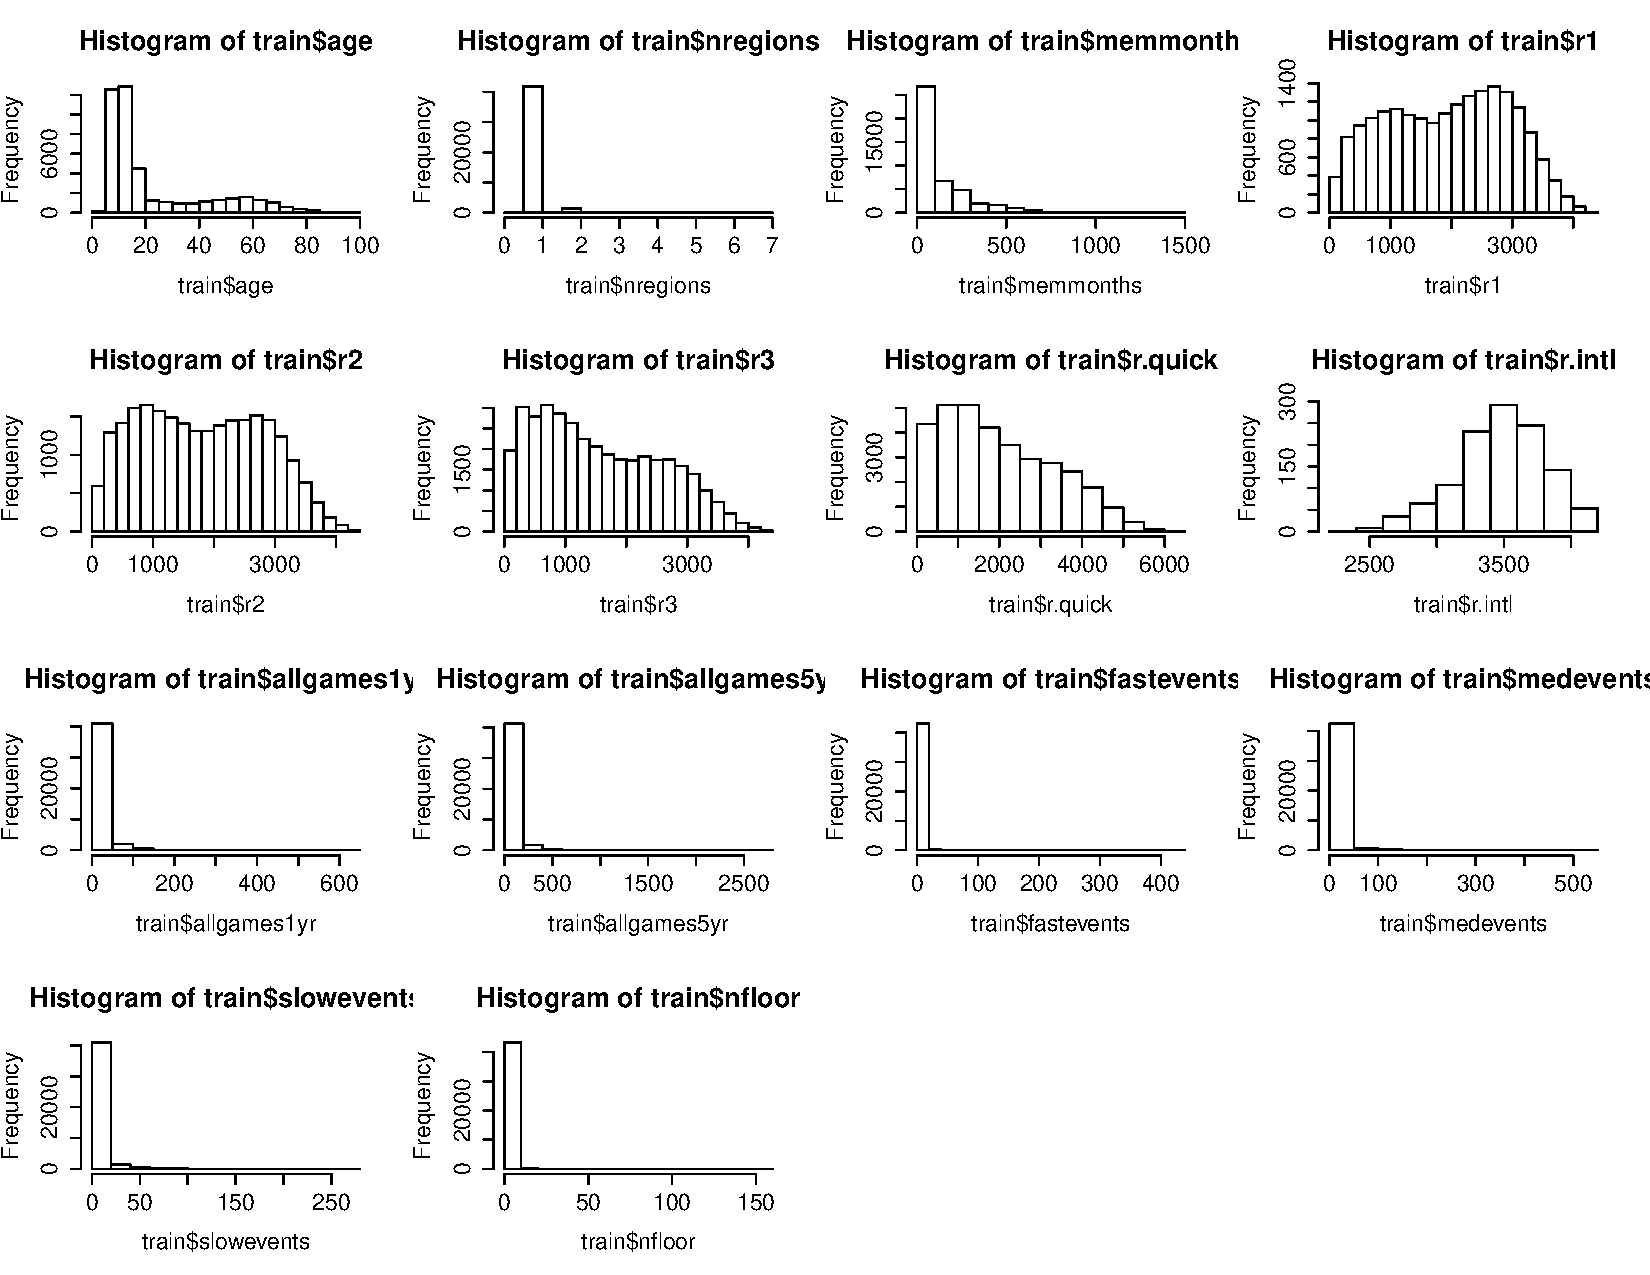
\includegraphics[width=\textwidth]{histograms_of_quant_vars}
    \caption{Histograms of Quantitative Predictors}
  \end{figure}
  \FloatBarrier

\section {Feature Engineering}
While we were provided with a number of helpful predictors, we felt there was an opportunity to create more powerful features from the data. We engineered four new features: the difference between an individual's $r3$ and $r2$ rating, the difference between an individual's $r2$ and $r1$ rating, the difference between an individual's $r3$ and $r.quick$ rating, and the average of an individual's $r1$, $r2$, and $r3$ (non-NA) ratings. We felt these new features help capture an individual's performance improvement over time (or lack thereof) over time which may be an indicator of whether or not an individual would be more likely to lapse.

\section*{Evolution of Models}
Here we outline the sequence of models we built and key insights that led us to change our approach with each model.
\begin{enumerate}
  \item 
  First, we made baseline predictions by fitting a generalized linear model (GLM) using the original features as the predictor variables.  Since we are trying to model a binary response variable, we fit a GLM from the binomial family, leveraging the logit as our link function. To find a best fitting logistic model, we used likelihood ratio tests to compare simpler models to more complex ones. We initially only considered single terms with no interactions, and built up a model by looking at the p value associated with the Chi Squared test statistic from our likelihood ratio test. If the p-value was less than 0.05, we would accept a more complex model over a simpler one. We also analyzed the change in deviance to prioritize the order by which we added statistically significant single terms to our GLM. This process was continued until all likelihood ratio tests showed that no more complex model was better.  When tested on 50\% of the test set, this model achieved a discrepancy of 0.56834. We were pleased with this result, as this simple model beat both baselines listed on Kaggle. 
  \item
  To improve upon our baseline predictions, we incorporated pairwise and three-way interaction terms between the following variables:age, number of regions, and number of months as a member.  Similar to the first, model we simplified the model as much as possible using likelihood ratio tests.  When tested on 50\% of the test set, this model achieved a discrepancy of 0.56529, an improvement of 0.00305 over the first model.
  \item
  We had observed that interaction terms were able to increase performance, but we hypothesized if a linear relationship between a predictor and the response was the most effective way to model the data. Thus, we felt it would be advantageous to instead use Generalized Additive Models (GAM), which we calculate a smoothing spline of quantitative variables, revealing any nonlinearities.  We again leveraged likelihood ratio tests to determine which predictors and smooths could be removed and which were statistically significant. When tested on 50\% of the test set, this model achieved a discrepancy of 0.54760, an improvement of 0.01769 over the previous model. 
  \item
  While our GAM approach was successful, we wanted to attempt to leverage the smoothers fit by the GAM to inform how we would fit a GLM with manual basis transformations of our predictor variables. Specifically, using smoothers reduce some of your data, thus if one knows the true transformation of the data (e.g., linear or quadratic), one should use that transformation using a GLM. In this way, the full data set would be used and we wouldn't be losing any information. Thus, to determine what non-linearities exist, we plotted the smoothing spline calculated for each quantitative variable and determined if the relationship was constant, linear, quadratic, or cubic. In Figure 2, we see that age, for example, appears to follow a cubic trend, thus we created new features that included age squared and age cubed (where we made sure to subtract out the mean of the predictor first to limit any unintended collinearity). Repeating this process for the other predictors that appeared to exhibit a non linear relationship, we built a logistic regression model that included single, pairwise, and triplet-wise interactions of all of our terms from the ground up using likelihood ratio tests. When tested on 50\% of the test set, this model achieved a discrepancy of 0.58, which was not an improvement. This is likely due to our interpretation of the smoothing splines to not be exactly correct, and thus the smooths themselves in a GAM were still more effective than our interpretation at this time.
  
    \item
  Our final approaches moved away from GLMs and GAMs altogether. We ran a random forest, tuned using cross validation, and a Neural Network. The Neural Network.... When tested on 50\% of the test set, this model achieved a discrepancy of 0.54, which was not an improvement. 
  
  
\end{enumerate}
  \FloatBarrier
  \begin{figure}[!ht]
    \centering
    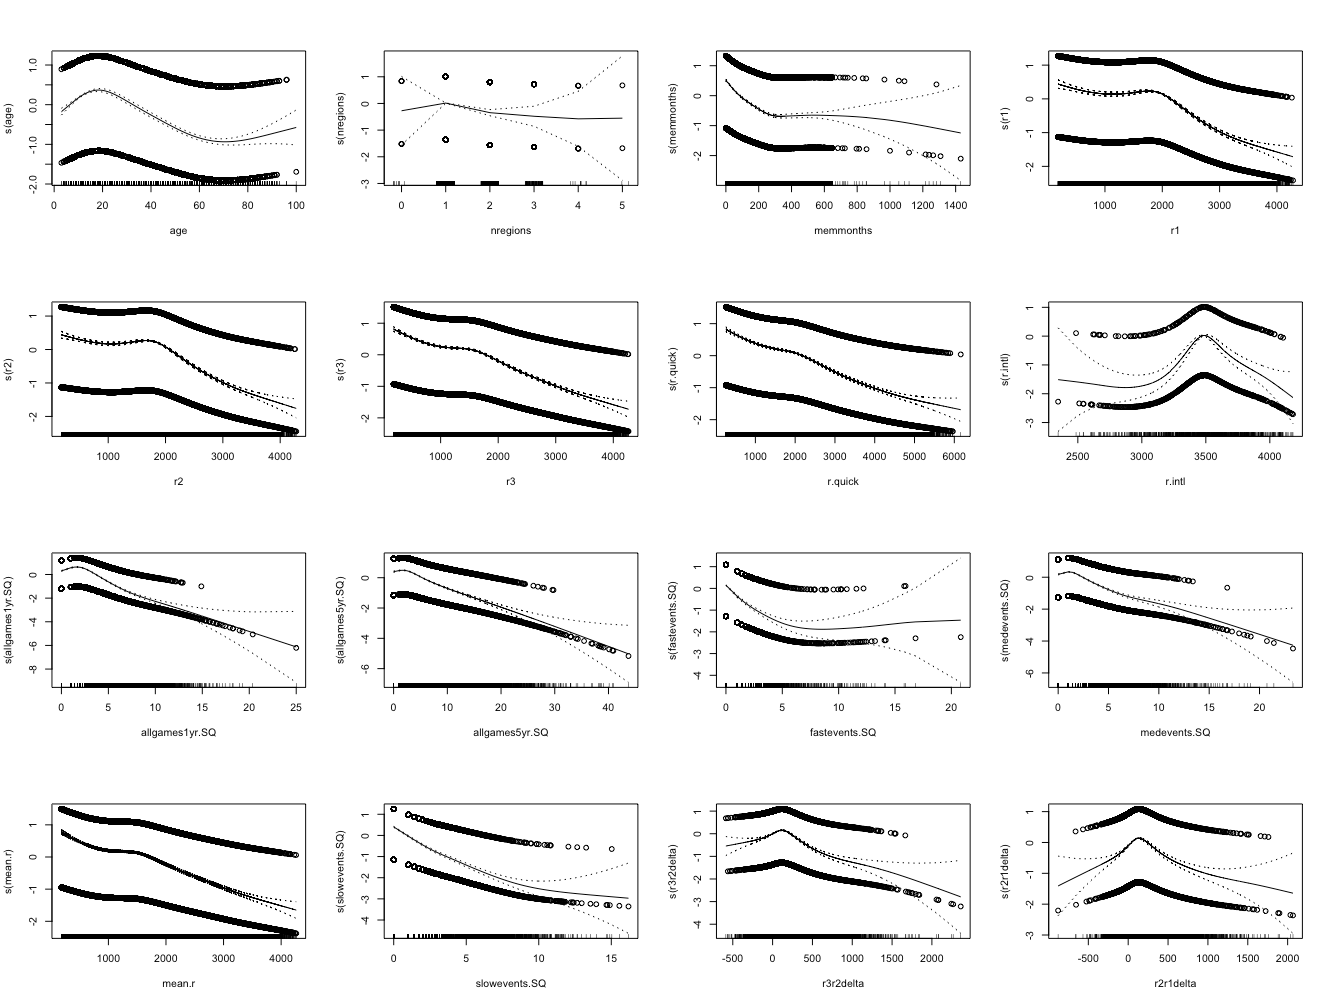
\includegraphics[width=\textwidth]{smoothers.png}
    \caption{Smoothers}
  \end{figure}
  \FloatBarrier
\section*{Analysis of Final Models}
We decided to move forward with our third and fifth models outlined above. First, we retrained our models on the full training set (reincorporating validation data into training data) so that we could leverage all the information available to us. Further, we ran some diagnostics to see if we have a model with a good fit. First, since the dispersion parameter for the binomial family is taken to be equal to 1, we can compare the residual deviance divided by the degrees of freedom and compare that value to the dispersion parameter. If it is close to 1, then we have a relatively good fitting model. In the included summary of our GAM model below, we see the fraction described is equal to 47163/43329 = 1.08, which is very close to one. Unfortunately, the coefficients of a GAM that incorporate smoothers are not interpretable like they typically are when using a GLM. 

We also plotted Cook's distances to see if any influential data points existed. From Fig 3, we see that no value is greater than 1, indicating that no influential points appear to exist. Another diagnostic we used leveraged the residuals of the data set. Specifically, we plotted Jack Knife residuals and Binned Average Residuals (Fig 4 and 5). From my Jack Knife plot, we see some observations are above and below 2 and -2. This indicates a poor fit. Since teh stripe shape is an artefact of our binary data, we also plotted binned average residuals. Here, we aim to have no non linearities present in the plot. However, from the fiture we see a trend that is not a horizontal line. Thus, this indicates we may have have a perfectly fitting model. 

\lstinputlisting[float=h,frame=tb,caption=GAM Model Summary,label=zebra, basicstyle=\tiny]{GAMsummary.txt}


  \FloatBarrier
  \begin{figure}[!ht]
    \centering
    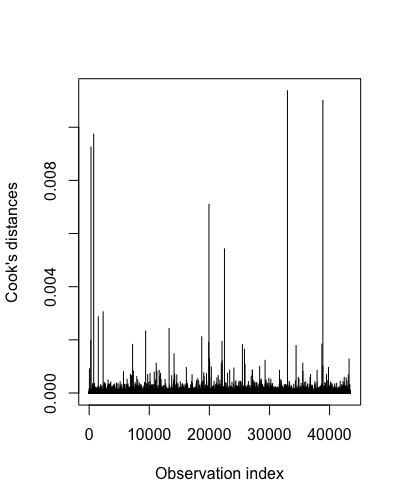
\includegraphics[scale=.5]{pp33.png}
    \caption{Cook's Distances}
  \end{figure}
  \FloatBarrier
  \FloatBarrier
  \begin{figure}[!ht]
    \centering
    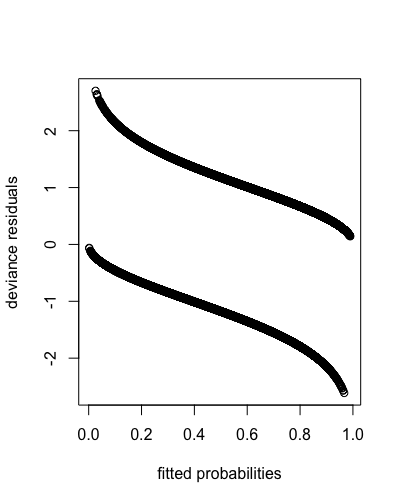
\includegraphics[scale=.5]{pp11.png}
    \caption{Jack Knife Residuals}
  \end{figure}
  \FloatBarrier

\FloatBarrier
  \begin{figure}[!ht]
    \centering
    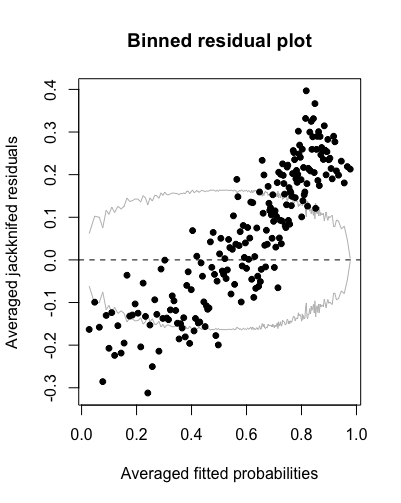
\includegraphics[scale=.5]{pp22.png}
    \caption{Binned Average Residuals}
  \end{figure}
  \FloatBarrier

\section*{Next Steps}
If we had additional time, we would have liked to run a RandomForest. We were able to run a preliminary model, which performed quite well, but we did run into a few snags. For example, we were unable to run a random Forest on the region predictor. this was unfortunate, as the region predictor appeared to be statistically significant in our other models. That said, our cross-validation technique was very helpful in tuning the number of trees in the forest before predicting on the test set (to avoid overfitting). Had we had more time to learn more about the benefits of Random Forests, we would have liked to further studied these and apply them to our modeling problem.

\end{document}